\section{Methodology}
\label{sec:methodology}
This section discusses the methodology used to obtain the results. First, the LCR-Rot-hop++ model is explained in detail. Thereafter, the four methods for document knowledge transfer (PRET, MULT, PRET+MULT, and PRET+MULT+FT) are elaborated upon. Last, the experimental setup for obtaining the results is given.
% \todo[inline]{Methodology: \textit{what kind of econometric methods and statistical techniques are you going to use to investigate the research problem? Why are those techniques suitable to address your research question(s)?}}

\subsection{LCR-Rot-hop++}

In this section we present the LCR-Rot-hop++ model \cite{Trusca2020}. This model is an extension of the LCR-Rot-hop model \cite{Wallaart2019}, and is consideed a state-of-the-art model for ABSC.

The BERT model is used to generate deep contextual word embeddings. The final representation of a word is calculated by summing its last four hidden states. We follow the approach of \cite{Trusca2020} in that we use the BERT-Base model with $L=12$ layers, $A=12$ attention heads, and $H=768$ hidden units. Each sentence is divided into the left context, the aspect (target), and the right context. The BERT word embeddings are divided accordingly into three embedding matrices, $S^l = [s_1^l,...,s_L^l]$, $S^t = [s_1^t,...,s_T^t]$, and $S^r = [s_1^r,...,s_R^r]$, where $s_i^j$ is the embedding for word $i$ in part $j$. Each embedding matrix is fed through the corresponding BiLSTM. This results in the hidden states, denoted as $H^l = [h_1^l,...,h_L^l]$, $H^t = [h_1^t,...,h_T^t]$, and $H^r = [h_1^r,...,h_R^r]$. The size of $h_i^j$ is a hyperparameter to be optimized, which we denote as the dimension $d$. 

Subsequently, the output from the left, center, and right BiLSTM are iteratively propagated through a rotatory attention mechanism. This iterative mechanism consists of two steps: Target2Context and Context2Target. The prior is used to obtain a representation from the context by focusing on specific words that are related to the target, hence, Target2Context. Afterward, this new context representation is used to acquire a better representation of the target itself, hence Context2Target. The newly obtained target representations in step 2 can be used to execute step 1, leading to an iterative process. Both steps are now explained in more detail.

\subsubsection{Step 1: Target2Context Attention Mechanism.}
First, an average target representation $r^{t_p}$ is computed using an average pooling layer over the vectors in $H^t$. Then, for both the left and the right context, an attention function $f$ is computed for each word to determine the level of focus. This attention function is defined as
\begin{equation}
    \undset{1\times 1}{f(h_i^l, r^{t_p})}=\mathrm{tanh}(\undset{1\times 2d}{h_i^{l'}}\times \undset{2d\times 2d}{W_c^l}\times \undset{2d\times 1}{r^{t_p}}+\undset{1\times 1}{b_c^l}),
\end{equation}
where $W_c^l$ is a weight matrix and $b_c^l$ is a bias. Next, these attention scores are normalized by applying the softmax function
\begin{equation}
    \alpha_i^l=\frac{\mathrm{exp}(f(h_i^l,r^{t_p}))}{\sum^L_{j=1} exp(f(h_j^l,r^{t_p}))}.
\end{equation}
Last, the left and right context are represented in a single vector by summing the weighted hidden states of the embedding matrix as follows
\begin{equation}
    \undset{2d\times 1}{r^l}=\sum^L_{i=1} \undset{1\times 1}{\alpha_i^l}\times \undset{2d\times 1}{h_i^l}.
\end{equation}
We compute $r^r$ in a similar fashion as $r^l$.

\subsubsection{Step 2. Context2Target Attention Mechanism.}
In the second step, we generate new target representations in a similar way, following the previous three equations, with the exception that we use $r^l$ and $r^r$ in place of $r^{t_p}$. This leads to two new target representations: one based on the left context and one based on the right context. The following equation denotes the left Context2Target representation
\begin{equation}
    \undset{2d\times 1}{r^{t_l}}=\sum_{i=1}^T \undset{1\times 1}{\alpha_i^{t_l}}\times \undset{2d\times 1}{h_i^t}.
\end{equation}
We again obtain the right Context2Target representation $r^{t_r}$ similarly as $r^{t_l}$.

In \cite{Wallaart2019}, the attention mechanism is improved by iteratively applying the steps. The newly obtained target representations in step 2 can be utilised to generate new attention scores in step 1. This extends the LCR-Rot model to the LCR-Rot-hop model, as each iteration of the attention mechanism is called a ``hop''. This is further improved in \cite{Trusca2020} by applying a hierarchical attention mechanism, the architecture of which is shown in Fig.  \ref{fig:haabsa++}.
\begin{figure}[h!]
    \centering
    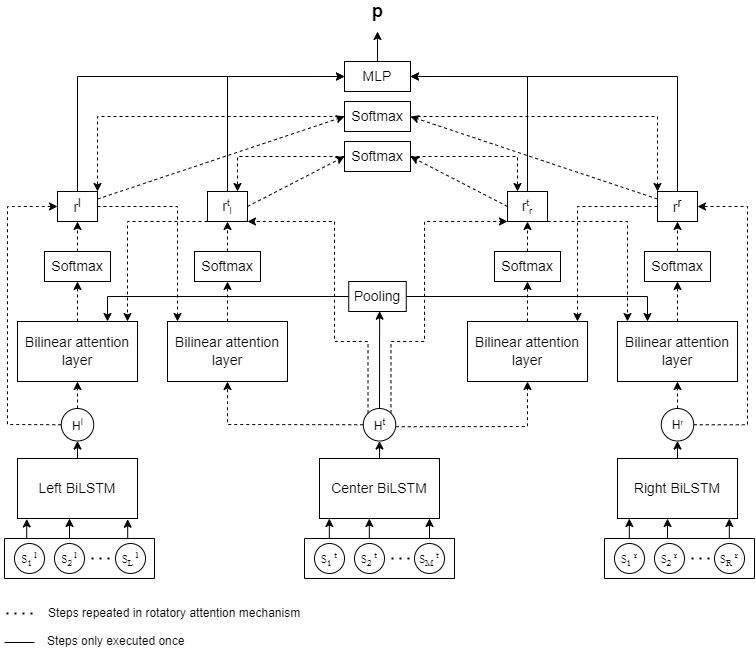
\includegraphics[width=\textwidth]{Images/LCR-Rot-Hop++.jpg}
    \caption{LCR-Rot-hop++ model}
    \label{fig:haabsa++}
\end{figure}

Hierarchical attention consists of scaling the Context\-2\-Target and Target\-2\-Context vectors using a sentence-level relevance score. Intuitively, the hierarchical attention decides whether more emphasis should be put on the left or right context. 
First, an attention function $f$ is computed, which is defined as
\begin{equation}
    \undset{1\times 1}{f(v^i)}=\mathrm{tanh}(\undset{1\times 2d}{v^{i'}}\times \undset{2d\times 1}{W}+\undset{1\times 1}{b}),
\end{equation}
where $v^i\in \{r^l, r^{t_l}, r^{t_r}, r^r\}$ is representation $i$ of the input sentence, $W$ is a weight matrix, and $b$ is a bias term. Then we compute new attention scores for each pair $\{r^l,r^r\}$ and $\{r^{t_l},r^{t_r}\}$ separately. The attention scores and newly obtained representations are defined as
\begin{equation}
    \alpha^i=\frac{\mathrm{exp}(f(v^i))}{\sum_{j=1}^2 \mathrm{exp}(f(v^j))},
\end{equation}
\begin{equation}
    \undset{2d\times 1}{v^i}=\undset{1\times 1}{\alpha^i}\times \undset{2d\times 1}{v^i}.
\end{equation}
As in \cite{Trusca2020}, we apply the attention weighting separately in each iteration of the rotatory attention mechanism, both on the pairs of intermediate context vectors and on the pairs of target vectors. In other words, after each Target2Context step, the hierarichal attention is applied to the $\{r^l,r^r\}$ pair, while after each Context2Target step, the hierarichal attention is applied to the $\{r^{t_l},r^{t_r}\}$ pair.

\subsection{Knowledge Transfer}
This paper considers several different approaches for document knowledge transfer. Each approach consists of one or more of the following building blocks: PRET, MULT, and FT. In this section, each building block will be described separately. Furthermore, Fig. \ref{fig:pretmultft} displays which compositions of PRET, MULT and FT are implemented in this paper. In the notation of each building block, we consider the two tasks $\tau_1$ and $\tau_2$. Let $\tau_2$ be our task of interest, namely ABSC. In contrast, $\tau_1$ is sentiment classification at a document level, which is semantically related to our main task. Therefore, teaching our model to execute $\tau_1$ will enlighten it with knowledge that can be used for better executing $\tau_2$. 

\begin{figure}[h!!!!!]
    \centering
    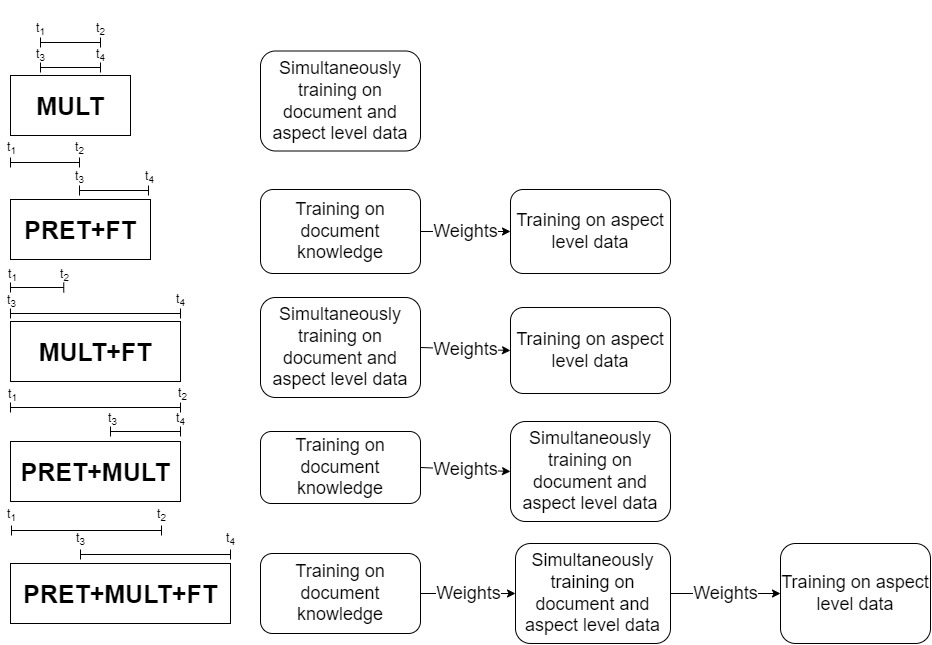
\includegraphics[width=\textwidth]{Images/PRET_MULT.jpg}
    \caption{An overview of the different document knowledge transfer approaches. The target task is executed in the time interval $[t_3, t_4]$, whereas the semantically related task is executed in the time interval $[t_1, t_2]$}
    \label{fig:pretmultft}
\end{figure}

\subsubsection{PRET.}
In the pretraining stage only $\tau_1$ is executed, which trains the model for sentiment analysis at a document level. Specifically, the documents are put through the left, center, and right BiLSTM, after which the final hidden layers of all words are pooled. The pooled hidden layers of the three BiLSTMs are concatenated and fed into a classification layer. The aim of this stage is to pretrain the BiLSTMs, as it is expected that the BiLSTM weights obtained in the PRET stage transfer the information from the document level sentiment classification to improve the accuracy at the aspect level.

\subsubsection{MULT.}
During the multi-task stage, tasks $\tau_1$ and $\tau_2$ are executed simultaneously.  In this approach, the three BiLSTMs are trained simultaneously on the document-level data and on their corresponding part of the aspect-level data (left, target, or right). Each aspect-level data point is paired to a document-level data point. Thus, the embedding layer and the three BiLSTMs in the LCR-Rot-hop++ model are shared for $\tau_1$ and $\tau_2$. The document-level data is processed the same as in the PRET stage. For the aspect-level data, the outputs from the BiLSTMs are directed to the corresponding attention mechanism, which finally leads to probabilities regarding the aspect-based sentiment.

% The data for $\tau_1$ can be propagated through both the left, right, and/or center BiLSTM of the LCR-Rot-hop++ model. After the BiLSTM outputs a document representation, it will be sent to a separate classification layer. In the end, the embedding layer and a number of the three BiLSTMs in the LCR-Rot-hop++ will be shared for $\tau_1$ and $\tau_2$. Table \ref{tab:MULT ways} shows the combinations which will be tested. 

% Please add the following required packages to your document preamble:
% \usepackage{booktabs}
%\begin{table}[htbp]
%\caption{}
%\label{tab:MULT ways}
%\begin{tabular}{@{}l@{}}
%\toprule
%\textbf{LSTM used for document sentiment %classification} \\ \midrule
%Left LSTM + right LSTM + center LSTM                     \\
%Left LSTM + right LSTM                                   \\
%Left LSTM                                                \\
%Right LSTM                                               \\ \bottomrule
%\end{tabular}
%\end{table}

The parameters are set by minimizing the loss function below.

\begin{equation}
    L = J + \lambda U + \omega \|\Theta\|_1 + \Omega  {\|\Theta\|_2}^2
\end{equation}
In this loss function, $J$ is the mean loss per training batch corresponding to our primary task $\tau_2$. Likewise, $U$ is the mean loss per training batch corresponding to our secondary task $\tau_1$. The loss $U$ is weighted with a parameter $\lambda \in (0,1)$, which can be interpreted as the importance of $\tau_1$ for performing $\tau_2$. Last, $\omega$ and $\Omega$ denote the weights of the L1 and L2 regularisation terms, respectively. The L1 regularisation considers the absolute value of the coefficients, whereas the L2 regularisation considers the squared coefficients. 

\subsubsection{FT.}
The fine-tuning stage can be used as the final stage for training a model. In the FT stage, only $\tau_2$ is executed. In this context, this means that only ABSC is performed. The goal of this stage is to tweak the model, such that it performs best for the target task. Whereas previous stages have taught the model more general knowledge, the FT stage aims at preparing the model solely for the target task.

\subsection{Experimental Setup}
To verify the added value of the TL approaches, we test all combinations as presented in Sect. 4.2 and compare their performance without document knowledge transfer. The following section describes in more detail how we find the best models for each combination.

\subsubsection{Hyperparameter Tuning.}

Hyperband is used to find the optimal hyperparameters \cite{Li2018}. As hypertuning all models over all stages is computationally infeasible, a heuristic  will be used for setting the hyperparameters. Namely, for each dataset, the optimal hyperparameters for the MULT model and the FT model are computed. These hyperparameters will be generalized over all building blocks of the model. Models which use hyperparameters from the tuned FT model are referred to as FT-based models. Models which use hyperparameters from the tuned MULT model are referred to as MULT-based models. Thus, each approach in Fig. 2 is executed using both the FT hyperparameters and the MULT hyperparameters. For the FT-based PRET+MULT+FT model, $\lambda$ has not been optimised in the hypertuning. Hence, the $\lambda$ from MULT tuning will be generalised to this model as well. Note that we do not run an FT-based model for MULT nor PRET+MULT, nor a MULT-based model for PRET+FT, as these parameter and TL approach combinations are likely to be suboptimal. 

\subsubsection{Model Training.}
Early stopping is applied to determine the number of training epochs with different levels of patience for the stages. This means that when the performance on the validation set has not increased during the patience epochs, the epochs after the current best epoch, training is stopped and the optimal model weights are restored. For the PRET stage, the performance measure is the validation loss (categorical cross-entropy). The PRET corpus is large compared to the aspect level data, so for computational efficiency a relatively low patience of 3 is chosen here. Similarly, for the MULT stage, we use early stopping with respect to the combined validation loss described in (8). We allow a higher patience of 10 as the per epoch time is considerably lower, making it more affordable. Last, for the FT stage, early stopping is done with respect to the validation accuracy, as this is our measure of interest. Again, a patience of 10 will be used. The loss functions in all stages, including the benchmark LCR-Rot-hop++, are regularised to prevent overfitting. Both L1 and L2 regularisation are used, the weights of which are optimised by the aforementioned hyperband for both FT-based and MULT-based models.

\subsubsection{Model Evaluation.}

We evaluate the various approaches using the out-of-sample accuracy measure. This measure allows us to see, after training, how often a model correctly predicts the sentiment of an aspect. We note that this measure weights the performance for each sentiment class according to how many observations there are for each sentiment, meaning it does not heavily penalise poor performance in a small sentiment class. As we observe in our data that there are very few neutral observations compared to positive and negative observations, we acknowledge that poor model performance when predicting a neutral sentiment might not be strongly reflected in the accuracy. For this reason, we also evaluate the models using a confusion matrix, to identify in which cases the model wrongly predicts the sentiment. A confusion matrix displays the predicted sentiment class and the corresponding observed sentiment class.

\subsubsection{Sensitivity Analysis.}

To analyse how sensitive the models are to both TL approaches, a sensitivity analysis is performed. First, PRET will be investigated; in particular, we will look at the effect of the size of the pretraining corpus on the model accuracy. Pretraining documents will be added in steps of 3000 up until 30000, our initial corpus. It could be that adding too many documents will lead to the model overfitting on our auxiliary task, whereas using too few documents might leave the model's knowledge lacking.

Additionally, the effect of the level of emphasis on the auxiliary task in MULT will be inspected. Mathematically, this means that we will increase $\lambda$ in (8) with steps of 0.1, starting at 0.1 up until 0.95. Higher values of $\lambda$ put a higher emphasis on the auxiliary task, whereas lower values deem the document classification of less importance. 